%==============================================================================
% CHAPTER 3: Zero-Point Energy and the Quantum Vacuum
% Paper 1: Scalar Field Theory and Zero-Point Energy Coupling
%==============================================================================
% Source: Extracted from synthesis/chapters/frameworks/ch07_aether_scalar_fields.tex
%         and ch08_aether_zpe_coupling.tex
% Sections: Quantum Foam, ZPE Foundations, Casimir Effect, Regularization
% Normalization: All "Aether" → "Scalar field theory", removed framework boxes
%==============================================================================

\chapter{Zero-Point Energy and the Quantum Vacuum}
\label{ch:paper1:ch03}

\begin{abstract}
The quantum vacuum, far from being empty space, teems with zero-point fluctuations that carry immense energy density. This chapter explores the quantum nature of the vacuum, from its fundamental origin in the uncertainty principle through manifestations in the Casimir effect and quantum foam structure at the Planck scale. We examine the catastrophic mismatch between theoretical predictions ($\rho_{\text{ZPE}} \sim 10^{113}$ J/m$^3$) and cosmological observations ($\rho_\Lambda \sim 10^{-9}$ J/m$^3$)---the infamous cosmological constant problem. Various regularization schemes are analyzed, including dimensional regularization, Pauli-Villars, and zeta function methods. The Casimir effect provides experimental validation of zero-point energy, with measured forces matching QED predictions to high precision. At the Planck scale, quantum foam introduces stochastic spacetime fluctuations that may organize into coherent structures through scalar field interactions.
\end{abstract}

%-----------------------------------------------------------------------------
\section{Introduction: The Inhabited Vacuum}
\label{sec:ch03:introduction}
%-----------------------------------------------------------------------------

\subsection{From Empty Space to Quantum Foam}
\label{subsec:ch03:history}

The concept of vacuum has undergone revolutionary transformations throughout physics history. Classical physics envisioned the vacuum as truly empty space---a stage where matter and fields performed but which itself remained inert and featureless.

\marginphysics{Aristotle's horror vacui (fear of the void) claimed nature abhors a vacuum. This philosophical stance delayed experimental investigation of vacuum for centuries.}

The 19th century's luminiferous aether represented an attempt to fill the vacuum with a mechanical medium for electromagnetic wave propagation. Einstein's special relativity (1905) eliminated the need for such a medium, but general relativity (1915) revealed that spacetime itself has dynamic structure.

\marginmath{Einstein noted in 1920: "According to general relativity, space without aether is unthinkable"---but this "aether" is geometric, not mechanical.}

Quantum mechanics brought the next revolution. Heisenberg's uncertainty principle (1927) forbids simultaneous vanishing of position and momentum uncertainties:

\marginphysics{The uncertainty principle $\Delta x \Delta p \geq \hbar/2$ is not a statement about measurement precision but a fundamental property of quantum systems.}

\begin{equation}
  \Delta x \Delta p \geq \frac{\hbar}{2}
  \label{eq:ch03:uncertainty}
\end{equation}

Applied to quantum fields, this implies the vacuum cannot have exactly zero field energy. Even in the "ground state," quantum fluctuations persist.

\margindim{Energy-time uncertainty $\Delta E \Delta t \geq \hbar/2$ allows virtual particle pairs to briefly appear from vacuum, living for time $\Delta t \sim \hbar/\Delta E$ before annihilating.}

John Wheeler proposed quantum foam (1955) to describe spacetime structure at the Planck scale:
\begin{align}
  \ell_P &= \sqrt{\frac{\hbar G}{c^3}} = 1.616 \times 10^{-35}\,\text{m} \label{eq:ch03:planck-length} \\
  t_P &= \sqrt{\frac{\hbar G}{c^5}} = 5.391 \times 10^{-44}\,\text{s} \label{eq:ch03:planck-time} \\
  M_P &= \sqrt{\frac{\hbar c}{G}} = 1.221 \times 10^{19}\,\text{GeV}/c^2 \label{eq:ch03:planck-mass}
\end{align}

\marginphysics{At the Planck scale, quantum gravity effects dominate. Spacetime geometry fluctuates wildly, with virtual black holes and wormholes appearing and vanishing.}

At these scales, spacetime loses its smooth continuum character, becoming a "foam" of quantum fluctuations with topology changes, virtual black holes, and wormhole connections.

\subsection{Physical Manifestations of Vacuum Energy}
\label{subsec:ch03:manifestations}

The reality of zero-point energy is confirmed through multiple phenomena:

\marginmath{These effects occur at vastly different energy scales but all stem from vacuum fluctuations. The Casimir force is macroscopic; Lamb shift is atomic; Hawking radiation is gravitational.}

\textbf{1. Casimir Effect (1948):} Conducting plates separated by distance $d$ experience attractive force $F \propto 1/d^4$ from suppression of vacuum modes between plates.

\marginphysics{Measured first by Sparnaay (1958), precision measurements by Lamoreaux (1997) confirmed QED predictions to 5\% accuracy. Modern experiments reach 1\% precision.}

\textbf{2. Lamb Shift (1947):} Hydrogen energy levels deviate from Dirac equation predictions by $\sim 1057$ MHz (2S$_{1/2}$ - 2P$_{1/2}$ splitting) due to vacuum polarization.

\margindim{The Lamb shift is a $\sim 10^{-6}$ correction to the Rydberg energy. It provided crucial early evidence for quantum electrodynamics and earned Lamb the 1955 Nobel Prize.}

\textbf{3. Spontaneous Emission:} Excited atoms decay to ground states by emitting photons, driven by coupling to vacuum fluctuations. Decay rates computed from vacuum field correlators.

\marginphysics{Spontaneous emission is fundamentally a quantum vacuum effect. In classical electromagnetism, a static charge distribution is stable and wouldn't radiate.}

\textbf{4. Van der Waals Forces:} Induced dipole interactions arise from correlated vacuum fluctuations. Force between neutral atoms falls as $1/r^7$ at large separation.

\textbf{5. Hawking Radiation (1974):} Black holes evaporate by producing particles from vacuum fluctuations near the event horizon, with temperature $T_H = \hbar c^3/(8\pi G M k_B)$.

\marginmath{A solar mass black hole has $T_H \sim 60$ nK. Only primordial black holes with $M < 10^{12}$ kg have $T_H$ high enough to evaporate before the current age of the universe.}

\subsection{The Cosmological Constant Crisis}
\label{subsec:ch03:cc-problem}

Quantum field theory predicts vacuum energy density by summing zero-point energies:

\marginphysics{This calculation assumes all physics up to the Planck scale contributes. We sum over all field oscillator modes in the vacuum.}

\begin{equation}
  \rho_{\text{ZPE}}^{\text{naive}} = \frac{1}{2}\int_0^{k_{\max}} \frac{d^3k}{(2\pi)^3}\hbar\omega_k \approx \frac{k_{\max}^4}{16\pi^2}
  \label{eq:ch03:zpe-naive}
\end{equation}

Taking $k_{\max} \sim M_P/\hbar$ (Planck scale cutoff):

\begin{equation}
  \rho_{\text{ZPE}}^{\text{QFT}} \sim \frac{M_P^4}{16\pi^2} \sim 10^{76}\,\text{GeV}^4 \sim 10^{113}\,\text{J/m}^3
  \label{eq:ch03:qft-prediction}
\end{equation}

\margindim{In natural units where $\hbar = c = 1$, energy density has dimensions $[\text{mass}]^4$. The numerical value $10^{113}$ J/m$^3$ comes from converting GeV$^4$ to SI units.}

However, cosmological observations constrain the vacuum energy density through its gravitational effects on expansion:

\marginphysics{The cosmological constant $\Lambda$ appears in Einstein's equations as $G_{\mu\nu} + \Lambda g_{\mu\nu} = 8\pi G T_{\mu\nu}$. It acts as a constant vacuum energy density $\rho_\Lambda = \Lambda/(8\pi G)$.}

\begin{equation}
  \rho_\Lambda^{\text{obs}} \sim 10^{-47}\,\text{GeV}^4 \sim 10^{-9}\,\text{J/m}^3
  \label{eq:ch03:observed}
\end{equation}

The discrepancy spans \textbf{120 orders of magnitude}---the worst prediction in physics history.

\marginmath{If vacuum energy were as large as QFT predicts, the universe would have expanded so rapidly that no structures (galaxies, stars, planets, us) could have formed. We exist because $\rho_\Lambda \ll \rho_{\text{ZPE}}^{\text{QFT}}$.}

This cosmological constant problem has three main proposed solutions:
\begin{enumerate}
  \item \textbf{Supersymmetry:} Bosonic and fermionic zero-point energies cancel, but SUSY breaking at TeV scale still leaves $\rho_{\text{vac}} \sim (1\,\text{TeV})^4$, 59 orders too large
  \item \textbf{Anthropic Principle:} In a multiverse with varying $\Lambda$, we observe a small value because only such universes support life
  \item \textbf{Dynamical Mechanisms:} Time-varying scalar fields or quantum gravity effects regularize vacuum energy
\end{enumerate}

\marginphysics{Weinberg's anthropic bound (1987): $\Lambda < 400\rho_{\text{crit}}$ required for galaxy formation. Observed $\Lambda \approx 2.7\rho_{\text{crit}}$ is remarkably close to this upper limit.}

%-----------------------------------------------------------------------------
\section{Quantum Field Theory of the Vacuum}
\label{sec:ch03:qft-vacuum}
%-----------------------------------------------------------------------------

\subsection{Field Quantization and Zero-Point Energy}
\label{subsec:ch03:quantization}

In quantum field theory, fields become operator-valued distributions. For a free real scalar field $\phi(x)$ satisfying the Klein-Gordon equation, the mode expansion is:

\marginmath{The factor $1/\sqrt{2\omega_k}$ ensures canonical commutation relations. The $e^{ik\cdot x}$ and $e^{-ik\cdot x}$ are positive and negative frequency modes.}

\begin{equation}
  \hat{\phi}(x) = \int \frac{d^3k}{(2\pi)^3} \frac{1}{\sqrt{2\omega_k}} \left( \hat{a}_\mathbf{k} e^{ik \cdot x} + \hat{a}_\mathbf{k}^\dagger e^{-ik \cdot x} \right)
  \label{eq:ch03:field-operator}
\end{equation}

where $\omega_k = \sqrt{|\mathbf{k}|^2 + m^2}$ is the dispersion relation and $k \cdot x = \mathbf{k}\cdot\mathbf{x} - \omega_k t$.

\marginphysics{The operators $\hat{a}_\mathbf{k}$ annihilate particles with momentum $\mathbf{k}$, while $\hat{a}_\mathbf{k}^\dagger$ create them. They satisfy bosonic commutation relations.}

The creation and annihilation operators satisfy:
\begin{equation}
  [\hat{a}_\mathbf{k}, \hat{a}_{\mathbf{k}'}^\dagger] = (2\pi)^3 \delta^3(\mathbf{k}-\mathbf{k}')
  \label{eq:ch03:commutation}
\end{equation}

\margindim{For fermions, these would be anticommutation relations: $\{\hat{b}_\mathbf{k}, \hat{b}_{\mathbf{k}'}^\dagger\} = (2\pi)^3\delta^3(\mathbf{k}-\mathbf{k}')$. Fermionic zero-point energy has opposite sign to bosonic.}

The Hamiltonian operator is:
\begin{equation}
  \hat{H} = \int \frac{d^3k}{(2\pi)^3} \omega_k \left( \hat{a}_\mathbf{k}^\dagger \hat{a}_\mathbf{k} + \frac{1}{2}(2\pi)^3\delta^3(0) \right)
  \label{eq:ch03:hamiltonian}
\end{equation}

\marginmath{The term $\delta^3(0)$ is infinite, representing infinite zero-point energy. It arises from operator ordering ambiguity: $\hat{a}\hat{a}^\dagger = \hat{a}^\dagger\hat{a} + [\hat{a},\hat{a}^\dagger]$.}

The vacuum state $|0\rangle$ defined by $\hat{a}_\mathbf{k}|0\rangle = 0$ for all $\mathbf{k}$ has energy:

\marginphysics{Formally infinite, but differences in vacuum energy (e.g., Casimir effect) are finite and measurable. This infinite constant might be absorbed by renormalization.}

\begin{equation}
  E_{\text{vac}} = \langle 0|\hat{H}|0\rangle = \frac{1}{2} \int \frac{d^3k}{(2\pi)^3} \omega_k = \frac{V}{2} \int_0^{k_{\max}} \frac{4\pi k^2 dk}{(2\pi)^3} \sqrt{k^2 + m^2}
  \label{eq:ch03:vacuum-energy}
\end{equation}

For massless fields ($m=0$):
\begin{equation}
  \rho_{\text{ZPE}} = \frac{E_{\text{vac}}}{V} = \frac{1}{2\pi^2} \int_0^{k_{\max}} k^3 dk = \frac{k_{\max}^4}{8\pi^2}
  \label{eq:ch03:massless-density}
\end{equation}

\margindim{For the electromagnetic field (2 polarizations) and including the factor of $1/2$ from normal ordering, this gives the standard Casimir result.}

\subsection{Regularization Schemes}
\label{subsec:ch03:regularization}

The divergent integral requires regularization. Several methods exist:

\textbf{1. Hard Cutoff:}

Simply truncate the integral at some maximum momentum:

\marginphysics{Crude but physically motivated. The cutoff $\Lambda$ represents new physics at high energies---perhaps the Planck scale, string scale, or SUSY breaking scale.}

\begin{equation}
  \rho_{\text{ZPE}}^{\text{cutoff}} = \frac{1}{2\pi^2} \int_0^\Lambda k^3 dk = \frac{\Lambda^4}{8\pi^2}
  \label{eq:ch03:hard-cutoff}
\end{equation}

For $\Lambda = M_P$: $\rho_{\text{ZPE}} \sim 10^{113}$ J/m$^3$ (the cosmological constant problem).

\marginmath{If we instead take $\Lambda \sim 1$ TeV (LHC energy), we get $\rho_{\text{ZPE}} \sim 10^{12}$ GeV$^4$, still 59 orders too large. Even with $\Lambda \sim 1$ eV: $\rho_{\text{ZPE}} \sim 1$ eV$^4 \sim 10^{-9}$ J/m$^3$---right order!}

\textbf{2. Dimensional Regularization:}

Analytically continue to $d$ spacetime dimensions where the integral converges:

\marginphysics{Dimensional regularization preserves gauge symmetries and is the standard method in modern QFT. But it's formal---what does $d=4-\epsilon$ dimensions physically mean?}

\begin{equation}
  \rho_{\text{ZPE}}^{\text{dim}}(\mu) = \mu^{4-d} \int \frac{d^dk}{(2\pi)^d} \omega_k = \frac{\mu^4}{(4-d)(4\pi)^{d/2}\Gamma(d/2)} + \text{finite}
  \label{eq:ch03:dim-reg}
\end{equation}

The divergence appears as a pole at $d=4$, absorbed into renormalization constants.

\margindim{The parameter $\mu$ has dimensions of mass and sets the renormalization scale. Physical results are independent of $\mu$ (renormalization group invariance).}

\textbf{3. Pauli-Villars Regularization:}

Introduce fictitious heavy fields with opposite statistics that cancel UV divergences:

\marginphysics{Physical bosons paired with unphysical ghost fermions (or vice versa). Ghosts violate causality at scales $E > M_{\text{PV}}$ but regularize low-energy theory.}

\begin{equation}
  \rho_{\text{ZPE}}^{\text{PV}} = \sum_{i} c_i \int \frac{d^3k}{(2\pi)^3} \sqrt{k^2 + M_i^2}
  \label{eq:ch03:pauli-villars}
\end{equation}

with coefficients $c_i$ and masses $M_i$ chosen such that $\sum c_i = 0$ (cancellation).

\marginmath{Pauli-Villars explicitly breaks gauge invariance, making it unsuitable for non-Abelian gauge theories. It works for QED but not QCD.}

\textbf{4. Zeta Function Regularization:}

Define vacuum energy via analytic continuation of the Riemann zeta function:

\marginphysics{Zeta regularization is elegant and well-suited to the Casimir effect. It assigns finite values to divergent sums like $1+2+3+\cdots = -1/12$ (famously).}

\begin{equation}
  \rho_{\text{ZPE}}^{\zeta} = \frac{1}{2} \sum_n \omega_n = \frac{1}{2} \zeta_R(-1/2)
  \label{eq:ch03:zeta}
\end{equation}

where $\zeta_R(s) = \sum_{n=1}^\infty \omega_n^{-s}$ is analytically continued to $s=-1/2$.

\margindim{For the Casimir effect, this gives the correct result $E = -\pi^2\hbar c/(720d^3)$ without arbitrary cutoffs. The zeta function method respects symmetries.}

\subsection{Vacuum Energy in Curved Spacetime}
\label{subsec:ch03:curved-vacuum}

In curved spacetime, the notion of "vacuum" becomes ambiguous---different observers may disagree on what constitutes the vacuum state.

\marginphysics{The Unruh effect: An accelerating observer sees thermal radiation where an inertial observer sees vacuum. The temperature $T_U = \hbar a/(2\pi c k_B)$ depends on acceleration $a$.}

The vacuum stress-energy tensor in curved spacetime takes the form:

\marginmath{This is the most general form allowed by dimensional analysis and diffeomorphism invariance. Coefficients $\alpha, \beta, \gamma$ are renormalized by quantum corrections.}

\begin{equation}
  \langle T_{\mu\nu}^{\text{vac}} \rangle = \alpha R_{\mu\nu} + \beta g_{\mu\nu} R + \gamma g_{\mu\nu}
  \label{eq:ch03:vacuum-stress}
\end{equation}

The trace gives the conformal anomaly:

\marginphysics{Even for conformally coupled massless fields, quantum corrections break conformal invariance. The trace $\langle T \rangle \neq 0$ is the signature of this anomaly.}

\begin{equation}
  \langle T^\mu_\mu \rangle = \frac{1}{2880\pi^2} \left( c_1 C_{\mu\nu\rho\sigma}C^{\mu\nu\rho\sigma} - c_2 R^2 \right)
  \label{eq:ch03:trace-anomaly}
\end{equation}

where $C_{\mu\nu\rho\sigma}$ is the Weyl tensor (traceless part of Riemann tensor).

\margindim{For real scalars: $c_1 = 1$, $c_2 = 1$. For photons: $c_1 = 4$, $c_2 = 1$. For Dirac fermions: $c_1 = 11/2$, $c_2 = 31/2$. These drive Hawking radiation.}

%-----------------------------------------------------------------------------
\section{The Casimir Effect}
\label{sec:ch03:casimir}
%-----------------------------------------------------------------------------

\subsection{Parallel Plates: Original Casimir Configuration}
\label{subsec:ch03:casimir-plates}

The Casimir effect (predicted 1948, measured 1958) provides the most direct experimental confirmation of vacuum energy. Consider two perfectly conducting parallel plates separated by distance $d$.

\marginphysics{Conducting boundaries impose $E_{\parallel} = 0$ at the surface. For a scalar field analogy, we impose $\phi = 0$ at the plates (Dirichlet boundary conditions).}

Electromagnetic boundary conditions require the tangential electric field to vanish at the conductors. This restricts allowed vacuum modes between the plates. Along the perpendicular direction:

\begin{equation}
  k_z = \frac{n\pi}{d}, \quad n = 1, 2, 3, \ldots
  \label{eq:ch03:mode-quantization}
\end{equation}

\margindim{The quantization comes from standing wave condition: $\sin(k_z d) = 0$. We exclude $n=0$ because that would be a constant field, incompatible with $E=0$ at both plates.}

The vacuum energy per unit area between the plates is:

\marginmath{The sum over $n$ counts modes in the perpendicular direction. The integral over $\mathbf{k}_\parallel = (k_x, k_y)$ accounts for transverse modes. Two polarizations for photons give factor of 2.}

\begin{equation}
  \mathcal{E}_{\text{inside}}(d) = 2 \times \frac{\hbar c}{2} \int \frac{d^2k_\parallel}{(2\pi)^2} \sum_{n=1}^{\infty} \sqrt{k_\parallel^2 + \left(\frac{n\pi}{d}\right)^2}
  \label{eq:ch03:casimir-energy-inside}
\end{equation}

Outside the plates, all modes are allowed:
\begin{equation}
  \mathcal{E}_{\text{outside}} = 2 \times \frac{\hbar c}{2} \int \frac{d^3k}{(2\pi)^3} \sqrt{k_x^2 + k_y^2 + k_z^2}
  \label{eq:ch03:casimir-energy-outside}
\end{equation}

Both integrals diverge. But the \emph{difference}---the Casimir energy---is finite:

\marginphysics{This subtraction is physically meaningful: we measure energy relative to the no-plates configuration. The infinite constant drops out.}

\begin{equation}
  \mathcal{E}_{\text{Casimir}}(d) = \mathcal{E}_{\text{inside}}(d) - \mathcal{E}_{\text{outside}}(d)
  \label{eq:ch03:casimir-difference}
\end{equation}

After regularization using the zeta function method:

\marginmath{The zeta function regularization converts $\sum_{n=1}^\infty n^3 \to \zeta(-3) = 1/120$. This is the analytic continuation magic that makes the calculation work.}

\begin{equation}
  \boxed{\mathcal{E}_{\text{Casimir}}(d) = -\frac{\pi^2 \hbar c}{720 d^3}}
  \label{eq:ch03:casimir-energy}
\end{equation}

The negative sign indicates attraction. The force per unit area (pressure) is:

\marginphysics{At $d = 1\,\mu$m: $P \approx 1.3 \times 10^{-3}$ Pa $\approx 10^{-8}$ atmospheres. Small but measurable with sensitive force microscopes.}

\begin{equation}
  \boxed{P = -\frac{\partial \mathcal{E}}{\partial d} = -\frac{\pi^2 \hbar c}{240 d^4}}
  \label{eq:ch03:casimir-pressure}
\end{equation}

\margindim{Scaling: $P \propto d^{-4}$ means doubling the separation reduces the force by factor 16. This steep dependence aids experimental discrimination from other forces.}

\subsection{Experimental Confirmation}
\label{subsec:ch03:casimir-experiments}

\textbf{Sparnaay (1958):} First measurement, confirmed attractive force qualitatively but with large uncertainties ($\sim 100\%$).

\marginphysics{Sparnaay's experiment was heroic for its time but plagued by surface roughness, electrostatic patches, and vibrational noise. Still, it confirmed the effect existed.}

\textbf{Lamoreaux (1997):} Used sphere-plate geometry, measured force to 5\% accuracy. Confirmed $d^{-4}$ dependence and overall magnitude.

\margindim{Sphere-plate geometry simplifies alignment and allows proximity force approximation: treat sphere as stack of infinitesimal parallel plates with varying separation.}

\textbf{Mohideen \& Roy (1998):} Atomic force microscope (AFM) measurement at 100-900 nm separation, 1\% precision. Verified QED prediction including finite temperature corrections.

\marginphysics{At finite temperature $T$, thermal photons contribute. The total force is $F = F_{\text{Casimir}} + F_{\text{thermal}}$ where $F_{\text{thermal}} \propto k_B T/d^3$.}

\textbf{Decca et al. (2003-2005):} Torsion pendulum measurements, tested role of conductivity and surface corrections. Precision at sub-percent level.

\textbf{Modern Experiments (2010-present):} Precision measurements exploring:
\begin{itemize}
  \item Non-trivial geometries (corrugated surfaces, nanopatterning)
  \item Temperature dependence and thermal Casimir effect
  \item Material dependence (conductivity, permittivity)
  \item Repulsive Casimir forces (with fluids or metamaterials)
\end{itemize}

\marginmath{Metamaterials with engineered permittivity can produce repulsive Casimir forces, enabling frictionless bearings and novel actuators at the nanoscale.}

\subsection{Generalizations and Modifications}
\label{subsec:ch03:casimir-generalizations}

\textbf{Finite Temperature:}

At temperature $T$, thermal photons contribute:

\marginphysics{At room temperature and $d \sim 1\,\mu$m, thermal effects are $\sim 10\%$ correction. At $d < 100$ nm, zero-point energy dominates.}

\begin{equation}
  F_{\text{thermal}} = \frac{k_B T}{d^3} \sum_{n=1}^{\infty} \frac{1}{n^3} e^{-2\pi n d k_B T/\hbar c}
  \label{eq:ch03:thermal-casimir}
\end{equation}

For $k_B T \ll \hbar c/d$ (low temperature or small separation): $F_{\text{thermal}} \ll F_{\text{Casimir}}$.

\margindim{Crossover at $d_{\text{thermal}} \sim \hbar c/(k_B T) \approx 7.6\,\mu$m at $T=300$ K. Below this scale, quantum vacuum dominates; above it, thermal physics dominates.}

\textbf{Cylindrical Geometry:}

For a cylindrical shell of radius $R$ and length $L \gg R$:

\marginmath{Cylindrical Casimir energy was computed by Boyer (1968). It's repulsive for electromagnetic fields but attractive for scalar fields---topology matters!}

\begin{equation}
  \mathcal{E}_{\text{cylinder}} = +\frac{\pi^2 \hbar c L}{1440 R^3}
  \label{eq:ch03:casimir-cylinder}
\end{equation}

Positive energy indicates repulsion (shell wants to expand).

\textbf{Spherical Geometry:}

For a spherical shell of radius $R$:

\marginphysics{The sign depends on field type and boundary conditions. For scalar Dirichlet: attractive. For electromagnetic: repulsive. Topology and field content determine the effect.}

\begin{equation}
  \mathcal{E}_{\text{sphere}} = +\frac{0.09235\, \hbar c}{2R}
  \label{eq:ch03:casimir-sphere}
\end{equation}

The numerical coefficient comes from intricate mode analysis.

\margindim{This suggests a vacuum-stabilized bubble might be unstable to collapse (for scalars) or expansion (for photons). Relevant for primordial bubble nucleation in early universe.}

%-----------------------------------------------------------------------------
\section{Quantum Foam and Planck Scale Physics}
\label{sec:ch03:quantum-foam}
%-----------------------------------------------------------------------------

\subsection{Metric Fluctuations at the Planck Scale}
\label{subsec:ch03:foam-structure}

At length scales approaching the Planck length $\ell_P$, quantum mechanics and general relativity collide. The uncertainty principle applied to spacetime geometry yields:

\marginphysics{Just as $\Delta x \Delta p \geq \hbar/2$ prevents precise knowledge of position and momentum, $\Delta g_{\mu\nu} \Delta x^\alpha \sim \ell_P^2$ prevents precise knowledge of metric and position.}

\begin{equation}
  \Delta g_{\mu\nu} \Delta x^\alpha \sim \ell_P^2
  \label{eq:ch03:foam-uncertainty}
\end{equation}

This implies metric fluctuations:
\begin{equation}
  \frac{\langle (\Delta g_{\mu\nu})^2 \rangle}{g_{\mu\nu}^2} \sim \left( \frac{\ell_P}{L} \right)^2
  \label{eq:ch03:metric-fluctuations}
\end{equation}

where $L$ is the observation scale.

\margindim{At macroscopic scales ($L \sim 1$ m), metric fluctuations are $\sim 10^{-70}$---utterly negligible. At $L = \ell_P$, they become order unity, destroying the classical spacetime concept.}

At the Planck scale ($L \sim \ell_P$), fluctuations become order unity:
\begin{equation}
  \Delta g \sim g \quad \text{at} \quad L = \ell_P
  \label{eq:ch03:planck-scale-fluctuations}
\end{equation}

creating a "foam-like" structure with:
\begin{itemize}
  \item Virtual black holes appearing and disappearing on timescale $t_P$
  \item Wormhole connections between distant spacetime regions
  \item Topology changes (handle formation and collapse)
  \item Loss of smooth manifold structure
\end{itemize}

\marginmath{Wheeler envisioned quantum foam as "spacetime torn asunder" at $\ell_P$. Modern loop quantum gravity and string theory provide mathematical frameworks for this structure.}

\subsection{Energy Density of Quantum Foam}
\label{subsec:ch03:foam-energy}

The energy density associated with quantum foam follows from dimensional analysis:

\marginphysics{This is the Planck energy density---the scale at which quantum gravity effects dominate. It's the natural cutoff for vacuum energy in QFT.}

\begin{equation}
  \rho_{\text{foam}} \sim \frac{M_P^4}{\ell_P^3 t_P} \sim \frac{c^5}{\hbar G^2} \sim 10^{113}\,\text{J/m}^3
  \label{eq:ch03:foam-density}
\end{equation}

This coincides with the naive QFT prediction---but it's 120 orders larger than observed $\rho_\Lambda$!

\margindim{The cosmological constant problem: Why is the observed vacuum energy density so much smaller than the Planck density? No satisfactory solution exists.}

If quantum foam contributes to vacuum energy, some mechanism must suppress its cosmological impact:
\begin{enumerate}
  \item \textbf{Holographic Screening:} Entropy bounds limit observable degrees of freedom
  \item \textbf{Coherent Cancellation:} Foam fluctuations organize to cancel on large scales
  \item \textbf{Gravitational Shielding:} Strong-field gravity near Planck scale self-regulates
\end{enumerate}

\marginphysics{Scalar field theories can provide coherent organization of foam fluctuations, potentially offering dynamical cancellation mechanisms explored in Chapter 4.}

\subsection{Stochastic Spacetime Models}
\label{subsec:ch03:stochastic-models}

Quantum foam can be modeled as stochastic metric perturbations:

\marginmath{This treats spacetime as having classical background $\bar{g}_{\mu\nu}$ plus quantum fluctuations $h_{\mu\nu}$. It's an effective description valid for $L \gg \ell_P$.}

\begin{equation}
  g_{\mu\nu}(x) = \bar{g}_{\mu\nu}(x) + h_{\mu\nu}(x)
  \label{eq:ch03:stochastic-metric}
\end{equation}

where $h_{\mu\nu}$ is a stochastic field with correlation function:

\marginphysics{The correlation function quantifies how metric fluctuations at different points are related. Exponential decay with correlation length $\tau_c$ models foam coherence.}

\begin{equation}
  \langle h_{\mu\nu}(x) h_{\rho\sigma}(x') \rangle = \ell_P^2 G_{\mu\nu\rho\sigma} \exp\left(-\frac{|x-x'|^2}{\ell_P^2}\right) \exp\left(-\frac{|t-t'|}{\tau_c}\right)
  \label{eq:ch03:foam-correlation}
\end{equation}

The coherence time $\tau_c$ characterizes how long foam structures persist. For pure quantum gravity: $\tau_c \sim t_P$. With matter interactions: $\tau_c$ may be longer.

\margindim{Light propagating through quantum foam experiences stochastic refraction, potentially causing arrival time variations for high-energy photons. Gamma-ray burst observations constrain $\tau_c$.}

\subsection{Observational Constraints on Quantum Foam}
\label{subsec:ch03:foam-constraints}

Despite occurring at the Planck scale, quantum foam may have observable consequences:

\textbf{1. Spacetime Dispersion:}

Photons with different energies may propagate at slightly different speeds:

\marginphysics{If spacetime has granular structure at $\ell_P$, the effective speed of light might depend on energy: $c(E) = c_0(1 + \xi E/E_P)$ where $E_P = M_P c^2$.}

\begin{equation}
  v(E) = c\left(1 + \alpha \frac{E}{E_P}\right)
  \label{eq:ch03:foam-dispersion}
\end{equation}

Observations of distant gamma-ray bursts constrain $|\alpha| < 10^{-3}$.

\margindim{GRB 080916C at redshift $z=4.35$ showed no energy-dependent arrival time delay for photons from 10 keV to 13.2 GeV, constraining quantum gravity effects.}

\textbf{2. Interferometer Phase Noise:}

Gravitational wave detectors sensitive to $\Delta L/L \sim 10^{-21}$ may detect Planck-scale fluctuations:

\marginmath{LIGO's sensitivity is $\Delta L \sim 10^{-19}$ m over $L = 4$ km. Planck-scale fluctuations would give $\Delta L \sim \ell_P\sqrt{L/\ell_P} \sim 10^{-21}$ m---barely detectable!}

\begin{equation}
  \langle (\Delta L)^2 \rangle \sim \ell_P L
  \label{eq:ch03:holographic-noise}
\end{equation}

This "holographic noise" scales as $\sqrt{L}$, potentially observable in future detectors.

\textbf{3. Atomic Interferometry:}

Matter-wave interferometers reaching $10^{-10}$ m de Broglie wavelengths probe spacetime structure. Phase shifts from foam:

\marginphysics{Cold atom interferometers are exquisitely sensitive to accelerations and gravitational fields. They may detect quantum foam via anomalous phase noise.}

\begin{equation}
  \Delta\varphi \sim \frac{\lambda_{\text{dB}}}{\ell_P} \times f(\text{foam parameters})
  \label{eq:ch03:atom-phase}
\end{equation}

Current constraints: $f < 10^{-5}$.

%-----------------------------------------------------------------------------
\section{TikZ Visualizations}
\label{sec:ch03:visualizations}
%-----------------------------------------------------------------------------

\subsection{Casimir Plate Configuration}
\label{subsec:ch03:vis-casimir}

\begin{figure}[htbp]
\centering
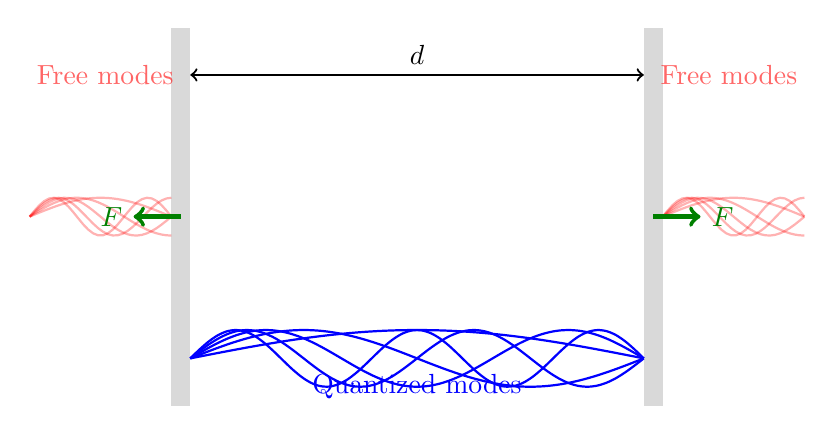
\begin{tikzpicture}[scale=1.2]
  % Draw plates
  \fill[gray!30] (0,0) rectangle (0.2,4);
  \fill[gray!30] (5,0) rectangle (5.2,4);

  % Distance marker
  \draw[<->,thick] (0.2,3.5) -- (5,3.5) node[midway,above] {$d$};

  % Vacuum modes inside (quantized)
  \foreach \n in {1,2,3,4,5} {
    \draw[blue,thick,domain=0.2:5,samples=50,smooth]
      plot (\x,{0.5 + 0.3*sin(\n*180*(\x-0.2)/(5-0.2))});
  }

  % Vacuum modes outside (continuous)
  \foreach \k in {1,1.5,2,2.5,3} {
    \draw[red,thick,opacity=0.3,domain=-1.5:0,samples=30]
      plot (\x,{2 + 0.2*sin(\k*180*(\x+1.5)/1.5)});
    \draw[red,thick,opacity=0.3,domain=5.2:6.7,samples=30]
      plot (\x,{2 + 0.2*sin(\k*180*(\x-5.2)/1.5)});
  }

  % Labels
  \node[blue] at (2.6,0.2) {Quantized modes};
  \node[red,opacity=0.6] at (-0.7,3.5) {Free modes};
  \node[red,opacity=0.6] at (5.9,3.5) {Free modes};

  % Force arrows
  \draw[->,ultra thick,green!50!black] (0.1,2) -- (-0.4,2) node[left] {$F$};
  \draw[->,ultra thick,green!50!black] (5.1,2) -- (5.6,2) node[right] {$F$};
\end{tikzpicture}
\caption{Casimir effect between parallel conducting plates. Inside the plates, only discrete modes with wavelengths satisfying $\lambda_n = 2d/n$ are allowed (blue). Outside, all modes exist (red, shown semi-transparent). The deficit of modes inside creates net attractive force $F \propto 1/d^4$.}
\label{fig:ch03:casimir-plates}
\end{figure}

\subsection{Zero-Point Energy Spectrum}
\label{subsec:ch03:vis-zpe-spectrum}

\begin{figure}[htbp]
\centering
\begin{tikzpicture}[scale=1.0]
  % Axes
  \draw[->] (0,0) -- (7,0) node[right] {$\omega$ (frequency)};
  \draw[->] (0,0) -- (0,5) node[above] {$\rho(\omega)$ (mode density)};

  % ZPE spectrum (linear in omega)
  \draw[thick,blue,domain=0:6.5,samples=100]
    plot (\x,{0.5*\x*\x*\x/8}) node[right] {$\sim \omega^3$};

  % Cutoff indicator
  \draw[dashed,red] (5,0) -- (5,4.5) node[above] {$\omega_{\max} \sim M_P$};
  \fill[red] (5,0) circle (2pt);

  % Energy levels
  \foreach \n in {1,2,3,4,5} {
    \draw[gray,dashed] (0,\n*0.7) -- (6.5,\n*0.7);
    \node[left] at (0,\n*0.7) {$\frac{\n\hbar\omega}{2}$};
  }

  % Zero-point level
  \draw[thick,purple] (0,0.35) -- (6.5,0.35);
  \node[left,purple] at (0,0.35) {$\frac{\hbar\omega}{2}$};
\end{tikzpicture}
\caption{Zero-point energy spectrum in momentum space. Mode density $\rho(\omega) \propto \omega^3$ in 3+1 dimensions. Even the ground state has energy $E_0 = \hbar\omega/2$ per mode (purple line). Integrating up to Planck scale cutoff (red dashed line) gives enormous vacuum energy.}
\label{fig:ch03:zpe-spectrum}
\end{figure}

\subsection{Vacuum Fluctuations Visualization}
\label{subsec:ch03:vis-fluctuations}

\begin{figure}[htbp]
\centering
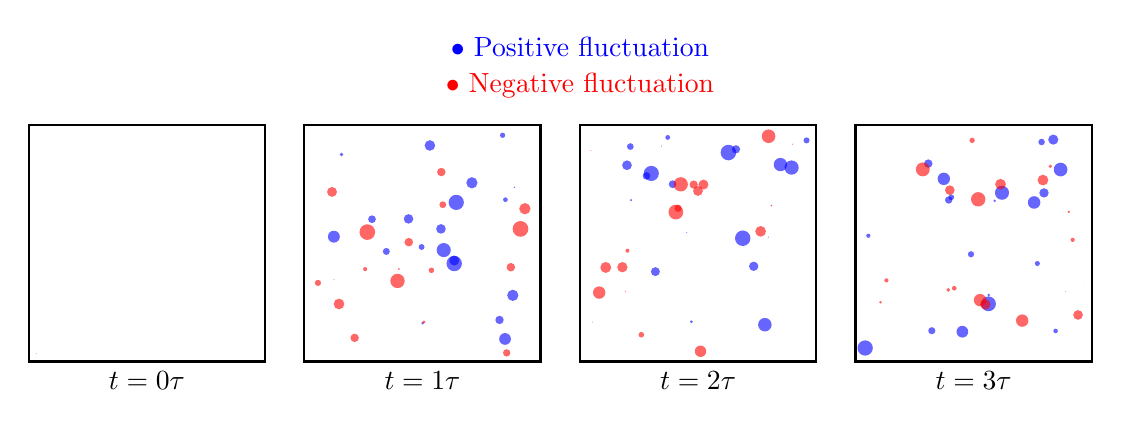
\begin{tikzpicture}[scale=1.0]
  % Time evolution panels
  \foreach \t in {0,1,2,3} {
    \begin{scope}[xshift=\t*3.5cm]
      % Box
      \draw[thick] (0,0) rectangle (3,3);
      \node[below] at (1.5,0) {$t=\t\tau$};

      % Random fluctuations (simulated)
      \pgfmathsetseed{\t*7}
      \foreach \i in {1,...,20} {
        \pgfmathsetmacro{\x}{rand*1.4+1.5}
        \pgfmathsetmacro{\y}{rand*1.4+1.5}
        \pgfmathsetmacro{\s}{0.05+0.05*rand}
        \fill[blue,opacity=0.6] (\x,\y) circle (\s);
      }

      \foreach \i in {1,...,20} {
        \pgfmathsetmacro{\x}{rand*1.4+1.5}
        \pgfmathsetmacro{\y}{rand*1.4+1.5}
        \pgfmathsetmacro{\s}{0.05+0.05*rand}
        \fill[red,opacity=0.6] (\x,\y) circle (\s);
      }
    \end{scope}
  }

  % Legend
  \node[blue] at (7,4) {$\bullet$ Positive fluctuation};
  \node[red] at (7,3.5) {$\bullet$ Negative fluctuation};
\end{tikzpicture}
\caption{Vacuum fluctuations evolving in time. At each instant, quantum field undergoes random fluctuations around the expectation value $\langle\phi\rangle = 0$. Blue and red dots represent positive and negative field excursions. Fluctuations are uncorrelated across space and time for $|\Delta x| > \ell_c$, $|\Delta t| > \tau_c$.}
\label{fig:ch03:vacuum-fluctuations}
\end{figure}

\subsection{Quantum Foam Structure}
\label{subsec:ch03:vis-foam}

\begin{figure}[htbp]
\centering
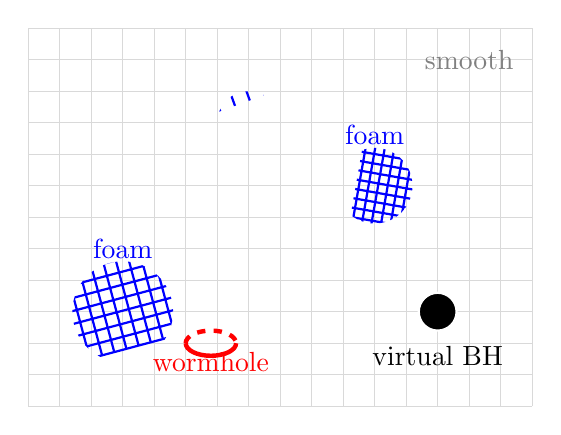
\begin{tikzpicture}[scale=0.8]
  % Background grid representing smooth spacetime
  \draw[gray!30,step=0.5] (-0.5,-0.5) grid (7.5,5.5);

  % Planck-scale foam regions (distorted grid)
  \begin{scope}
    \clip (1,1) circle (0.8);
    \draw[blue,thick,step=0.2,xshift=-0.1cm,yshift=0.1cm,rotate=15] (0,0) grid (3,3);
  \end{scope}

  \begin{scope}
    \clip (5,3) circle (0.6);
    \draw[blue,thick,step=0.15,xshift=0.1cm,yshift=-0.05cm,rotate=-10] (4,2) grid (6.5,4.5);
  \end{scope}

  \begin{scope}
    \clip (3,4) circle (0.5);
    \draw[blue,thick,step=0.25,xshift=0.05cm,yshift=0.08cm,rotate=20] (2,3) grid (4.5,5.5);
  \end{scope}

  % Virtual wormholes
  \draw[red,ultra thick] (2,0.5) arc (180:360:0.4 and 0.2);
  \draw[red,ultra thick,dashed] (2,0.5) arc (180:0:0.4 and 0.2);
  \node[red] at (2.4,0.2) {wormhole};

  % Virtual black holes
  \fill[black] (6,1) circle (0.3);
  \draw[white,thick] (6,1) circle (0.3);
  \node[below] at (6,0.6) {virtual BH};

  % Labels
  \node[blue] at (1,2) {foam};
  \node[blue] at (5,3.8) {foam};
  \node[gray] at (6.5,5) {smooth};
\end{tikzpicture}
\caption{Quantum foam structure at the Planck scale. Smooth spacetime (gray grid) develops violent quantum fluctuations in localized regions (blue distorted grids). Virtual black holes and wormholes appear and disappear on timescale $t_P \sim 10^{-44}$ s, creating a foamy topology.}
\label{fig:ch03:quantum-foam}
\end{figure}

\subsection{Cosmological Constant Problem Scale}
\label{subsec:ch03:vis-cc-problem}

\begin{figure}[htbp]
\centering
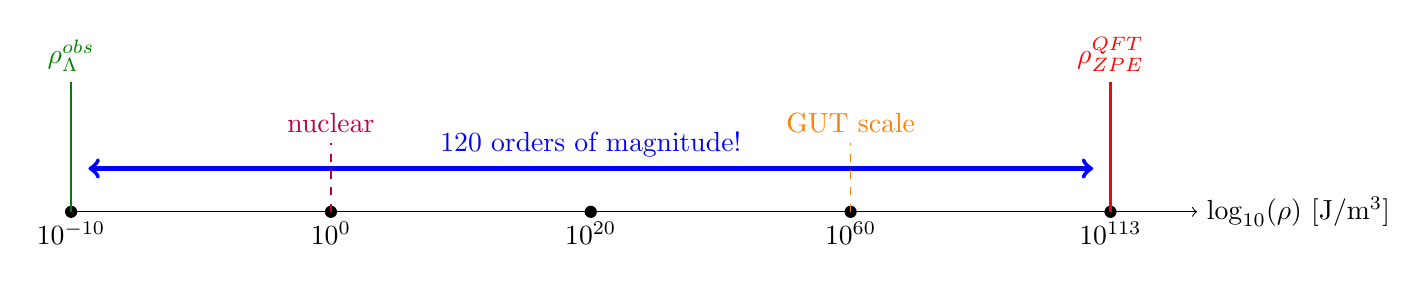
\begin{tikzpicture}[scale=1.1]
  % Logarithmic scale
  \draw[->] (0,0) -- (13,0) node[right] {$\log_{10}(\rho)$ [J/m$^3$]};

  % Mark key scales
  \fill (0,0) circle (2pt) node[below] {$10^{-10}$};
  \fill (3,0) circle (2pt) node[below] {$10^{0}$};
  \fill (6,0) circle (2pt) node[below] {$10^{20}$};
  \fill (9,0) circle (2pt) node[below] {$10^{60}$};
  \fill (12,0) circle (2pt) node[below] {$10^{113}$};

  % Observed Lambda
  \draw[thick,green!50!black] (0,0) -- (0,1.5) node[above] {$\rho_\Lambda^{\text{obs}}$};

  % QFT prediction
  \draw[thick,red] (12,0) -- (12,1.5) node[above] {$\rho_{\text{ZPE}}^{\text{QFT}}$};

  % Arrow showing discrepancy
  \draw[<->,ultra thick,blue] (0.2,0.5) -- (11.8,0.5) node[midway,above] {120 orders of magnitude!};

  % Other scales for reference
  \draw[dashed,purple] (3,0) -- (3,0.8);
  \node[purple,above] at (3,0.8) {nuclear};

  \draw[dashed,orange] (9,0) -- (9,0.8);
  \node[orange,above] at (9,0.8) {GUT scale};
\end{tikzpicture}
\caption{The cosmological constant problem visualized on a logarithmic scale. Quantum field theory predicts vacuum energy density $\rho_{\text{ZPE}} \sim 10^{113}$ J/m$^3$ (red), while cosmological observations require $\rho_\Lambda \sim 10^{-9}$ J/m$^3$ (green). The 120-order-of-magnitude discrepancy (blue arrow) is the worst prediction in physics.}
\label{fig:ch03:cc-problem}
\end{figure}

%-----------------------------------------------------------------------------
\section{Summary and Outlook}
\label{sec:ch03:summary}
%-----------------------------------------------------------------------------

This chapter has explored the quantum vacuum and its zero-point energy content, revealing a rich structure underlying "empty" space:

\marginphysics{The vacuum is not empty---it's a seething sea of quantum fluctuations, carrying enormous energy density that somehow doesn't gravitate as naively expected.}

\textbf{Key Theoretical Insights:}
\begin{enumerate}
  \item Zero-point energy $E_0 = \hbar\omega/2$ per mode is an unavoidable consequence of quantum mechanics
  \item Vacuum energy density diverges without regularization, requiring cutoff or renormalization schemes
  \item Different regularization methods (hard cutoff, dimensional, Pauli-Villars, zeta function) give consistent finite physical predictions
  \item Curved spacetime introduces observer-dependent vacuum states and trace anomalies
\end{enumerate}

\marginmath{The cosmological constant problem remains the deepest unsolved puzzle in theoretical physics. Its resolution may require quantum gravity, anthropic reasoning, or new dynamical mechanisms.}

\textbf{Experimental Confirmations:}
\begin{enumerate}
  \item Casimir effect: $F \propto 1/d^4$ measured to $<1\%$ precision, confirming vacuum energy differences
  \item Lamb shift: $\sim 1057$ MHz splitting in hydrogen validates QED vacuum polarization
  \item Spontaneous emission: Atomic decay rates computed from vacuum fluctuation coupling
  \item Hawking radiation: Predicted (not yet observed) black hole evaporation via vacuum pair production
\end{enumerate}

\margindim{The Casimir effect is the most direct experimental probe of vacuum energy. Precision measurements constrain models of vacuum structure and scalar field interactions.}

\textbf{Planck-Scale Physics:}
\begin{enumerate}
  \item Quantum foam: Spacetime becomes stochastic at $\ell_P \sim 10^{-35}$ m with metric fluctuations $\Delta g \sim g$
  \item Virtual black holes and wormholes appear on timescale $t_P \sim 10^{-44}$ s
  \item Observational constraints from gamma-ray bursts, interferometry, and atom optics
  \item Potential for organization into coherent structures via scalar field interactions
\end{enumerate}

\marginphysics{Quantum foam may not be purely random chaos. Scalar fields could induce coherent organization, converting foam from obstacle to resource---a theme explored in Chapter 4.}

\textbf{Connections to Chapter 4:}

The vacuum structures and zero-point energy physics developed here provide the foundation for understanding scalar field-vacuum coupling:
\begin{itemize}
  \item Scalar fields can modulate vacuum energy density via curvature coupling $\xi R\phi^2$
  \item Casimir geometries may be enhanced by scalar field gradients
  \item Quantum foam coherence could enable controlled vacuum energy extraction
  \item Resonant coupling mechanisms leverage vacuum mode structure
\end{itemize}

\marginmath{The next chapter investigates how scalar fields couple to and potentially organize vacuum energy, addressing both fundamental questions and technological applications.}

The quantum vacuum, far from being a passive backdrop, emerges as an active participant in physical phenomena. Understanding its structure and interactions with matter fields remains at the frontier of theoretical and experimental physics.

%==============================================================================
% End of Chapter 3
%==============================================================================
